\begin{enumerate}[label=\bfseries Câu \arabic*:]

\item \mkstar{1}

\cauhoi{
	
	Khi con ruồi và con muỗi bay, ta nghe được tiếng vo ve từ muỗi bay mà không nghe được từ ruồi là do
	\begin{mcq}(1)
		\item tần số đập cánh của muỗi thuộc vùng tai người nghe được.
		\item muỗi bay tốc độ chậm hơn ruồi.
		\item muỗi phát ra âm thanh từ cánh.
		\item muỗi đập cánh đều đặn hơn ruồi.
	\end{mcq}
}
\loigiai{
	
	\textbf{Đáp án A.}
	
	
	
	Khi con ruồi và con muỗi bay, ta nghe được tiếng vo ve từ muỗi bay mà không nghe được từ ruồi là do tần số đập cánh của muỗi thuộc vùng tai người nghe được.
	
	
	
	
	
}

\item \mkstar{1}

\cauhoi{
	
	Cho các chất sau: không khí ở $0^\circ \text{C}$, không khí ở $25^\circ \text{C}$, nước, sắt. Sóng âm truyền nhanh nhất trong môi trường nào?
	\begin{mcq}(2)
		\item Không khí ở $0^\circ \text{C}$.
		\item Nước.
		\item Sắt.
		\item Không khí ở $25^\circ \text{C}$.
	\end{mcq}
}
\loigiai{
	
	\textbf{Đáp án C.}
	
	
	
	Do vận tốc truyền âm trong chất rắn > chất lỏng > chất khí nên âm truyền trong sắt là nhanh nhất.
	
	
	
}
\item \mkstar{2}

\cauhoi{
	
	Hai âm cùng tần số có mức cường độ âm chênh lệch nhau là 15 dB. Tỉ số cường độ âm của chúng là
	\begin{mcq}(4)
		\item $120$.
		\item $1200$.
		\item $10\sqrt 10$.
		\item $10$.
	\end{mcq}
}
\loigiai{
	
	\textbf{Đáp án C.}
	
	$L_\text{A}-L_\text{B}=\log\dfrac{I_\text{A}}{I_\text{B}}\Rightarrow I_\text{A}=10\sqrt{10}I_\text{B}$.
	
	
	
	
}
\item \mkstar{2}

\cauhoi{
	
	Một âm có cường độ $5\cdot 10^{-7}\ \text{W/m}^2$. Mức cường độ âm của nó là
	\begin{mcq}(4)
		\item $\SI{37}{dB}.$
		\item $\SI{73}{dB}.$
		\item $\SI{57}{dB}.$
		\item $\SI{103}{dB}.$
	\end{mcq}
}
\loigiai{
	\textbf{Đáp án C.}
	
	$L=\log\dfrac{I}{I_0}=\SI{57}{dB}$.
	
}
\item \mkstar{2}

\cauhoi{
	
	Tại điểm A cách nguồn âm đẳng hướng $\SI{10}{m}$ có mức cường độ âm $\SI{24}{dB}$. Biết cường độ âm tại ngưỡng nghe là $I_0 = 10^{-12} \ \text{W/m}^2$. Vị trí có mức cường độ âm bằng 0 cách nguồn
	\begin{mcq}(4)
		\item xa vô cực.
		\item $\SI{3162}{m}$.
		\item $\SI{158,49}{m}$.
		\item $\SI{2812}{m}$.
	\end{mcq}	
}
\loigiai{
	
	\textbf{Đáp án C.}
	
	$L_\text{A}-L_\text{B}=10\log\dfrac{I_\text{A}}{I_\text{O}}-10\log\dfrac{I_\text{B}}{I_\text{O}}=\SI{24}{dB}\Rightarrow=\SI{158,49}{m}$.
	
	
	
	
}
\item \mkstar{2}

\cauhoi{
	
	Tại một điểm A nằm cách xa nguồn âm O (coi như nguồn điểm) một khoảng OA $=\SI{1}{cm}$, mức cường độ âm là $L_\text{A} =\SI{90}{dB}$. Cho biết ngưỡng nghe của âm chuẩn $I_0=10^{-12}\ \text{W/m}^2$. Coi môi trường là hoàn toàn không hấp thụ âm, mức cường độ âm tại B nằm trên đường OA cách O một khoảng 10 m là
	\begin{mcq}(4)
		\item $\SI{70}{dB}.$
		\item $\SI{50}{dB}.$
		\item $\SI{65}{dB}.$
		\item $\SI{75}{dB}.$
	\end{mcq}
}
\loigiai{
	
	\textbf{Đáp án A.}
	
	Ta có:
	
	$I_\text{A}=I_0 10^{L_\text{A}}=\dfrac{P}{4\pi\text{OA}^2}$.
	
	$I_\text{B}=I_0 10^{L_\text{B}}=\dfrac{P}{4\pi\text{OB}^2}$.
	
	Do đó: $10^{L_\text{A}-L_\text{B}}=\dfrac{\text{OB}^2}{\text{OA}^2}\Rightarrow L_\text{B}=L_\text{A}-\log\dfrac{\text{OB}^2}{\text{OA}^2}=\SI{70}{dB}$.
	
	
	
	
}
\item \mkstar{2}

\cauhoi{
	
	Một nguồn âm có công suất phát âm $P=\SI{0,1256}{W}$. Biết sóng âm phát ra là sóng cầu, cường độ âm chuẩn $I_0=10^{-12}\ \text{W/m}^2$. Tại một điểm trên mặt cầu có tâm là nguồn phát âm, bán kính 10 m (bỏ qua sự hấp thụ âm) có mức cường độ âm là
	
	\begin{mcq}(4)
		\item $\SI{90}{dB}.$
		\item $\SI{80}{dB}.$
		\item $\SI{60}{dB}.$
		\item $\SI{70}{dB}.$
	\end{mcq}
	
}

\loigiai{
	
	\textbf{Đáp án B.}
	
	$I=\dfrac{P}{4\pi r^2}\Rightarrow L=\log\dfrac{P}{4\pi r^2 I_0}=\SI{80}{dB}$.
	
	
	
	
}
\item \mkstar{2}

\cauhoi{
	
	Sóng cơ lan truyền trong không khí với cường độ đủ lớn, tai người bình thường không thể cảm thụ được sóng cơ nào sau đây?
	\begin{mcq}(2)
		\item Sóng cơ có chu kì 2 ms.
		\item Sóng cơ có tần số 100 Hz.
		\item Sóng cơ có tần số 0,3 kHz.
		\item Sóng cơ có chu kỳ $2\ \mu \text{s}$.
	\end{mcq}	
}
\loigiai{
	
	
	\textbf{Đáp án D.}
	
	Tai người bình thường chỉ nghe được âm có tần số khoảng từ $\SI{16}{Hz}$ đến $\SI{20000}{Hz}$.
	
	Sóng cơ có chu kì $2\ \mu \text{s}$ có tần số $f=\SI{500000}{Hz}$ nên tai người không thể cảm nhận được.
	
	
	
}
\item \mkstar{2}

\cauhoi{
	
	Ngưỡng đau của tai người khoảng $10\ \text{W/m}^2$. Một nguồn âm nhỏ đặt cách tai một khoảng $d=\SI{1}{m}$. Để không làm đau tai thì công suất tối đa của nguồn là
	\begin{mcq}(4)
		\item $\SI{125,6}{W}.$
		\item $\SI{12,5}{W}.$
		\item $\SI{11,6}{W}.$
		\item $\SI{1,25}{W}.$
	\end{mcq}
}
\loigiai{
	
	\textbf{Đáp án A.}
	
	Muốn không làm đau thì $I$ không vượt quá ngưỡng đau $\Rightarrow \dfrac{P}{4\pi d^2}<\SI{10}{W/m^2} \Rightarrow P<\SI{125,6}{W}$.
	
	
	
	
}
\item \mkstar{2}

\cauhoi{
	
	Một nguồn sóng âm (được coi như nguồn điểm) có công suất $1\ \mu \text{W}$. Cường độ âm và mức cường độ âm tại một điểm cách nguồn 3 m là
	\begin{mcq}(2)
		\item $\text{8,842}\cdot 10^{-9}\ \text{W/m}^2$; $\SI{39,465}{dB}.$.
		\item $\text{8,842}\cdot 10^{-9}\ \text{W/m}^2$; $\SI{394,65}{dB}.$.
		\item $\text{8,842}\cdot 10^{-10}\ \text{W/m}^2$; $\SI{3,9465}{dB}.$.
		\item $\text{8,842}\cdot 10^{-9}\ \text{W/m}^2$; $\SI{3,9465}{dB}.$.
	\end{mcq}	
}
\loigiai{
	
	\textbf{Đáp án A.}
	
	$I=\dfrac{P}{4\pi d^2}=\text{8,842}\cdot 10^{-9}\ \text{W/m}^2$.
	
	$L=\dfrac{I}{I_0}=\SI{39,465}{dB}$.
	
	
	
	
}

\item \mkstar{2}

\cauhoi{
	
	Vận tốc truyền âm trong không khí là 336 m/s. Khoảng cách giữa hai điểm gần nhau nhất trên cùng phương truyền sóng dao động vuông pha là 0,2 m. Tần số của âm là
	\begin{mcq}(4)
		\item 500 Hz.
		\item 400 Hz.
		\item 420 Hz.
		\item 840 Hz.
	\end{mcq}	
}
\loigiai{
	
	\textbf{Đáp án C.}
	
	Khoảng cách gần nhất giữa hai điểm dao động vuông pha: 
	
	$\Delta \varphi = \dfrac{\pi}{2} = \dfrac{\omega\cdot x}{v} = \dfrac{2\pi f\cdot x}{v}$. 
	
	$\Rightarrow$ $f=\dfrac{v}{4x}$ . 
	
	Thay số vào ta có: $f= \SI{420}{Hz}$.
	
	
}
\item \mkstar{2}

\cauhoi{
	
	Một sóng âm truyền trong không khí. Mức cường độ âm tại điểm M và tại điểm N lần lượt là $40$ dB và $70$ dB. Cường độ âm tại N lớn hơn cường độ âm tại M gấp
	\begin{mcq}(4)
		\item 10000 lần.
		\item 2 lần.
		\item 40 lần.
		\item 1000 lần.
	\end{mcq}
}
\loigiai{
	
	\textbf{Đáp án D.}
	
	
	Ta có:
	
	$L_\text{M}=10 \log\dfrac{I_\text{M}}{I_0} \Rightarrow I_\text{M}=10^{\frac{L_\text{M}}{10}}I_0\ (1)$
	
	$L_\text{N}=10\log\dfrac{I_\text{N}}{I_0}\Rightarrow I_\text{N}=10^{\frac{L_\text{N}}{10}}I_0\ (2)$
	
	Từ (1) và (2) suy ra:
	
	$\dfrac{I_\text{N}}{I_\text{M}}=\dfrac{10^{\frac{L_\text{N}}{10}}}{10^{\frac{L_\text{M}}{10}}}=10^{\frac{L_N-L_M}{10}}=1000$
	
	
}

\item \mkstar{2}

\cauhoi{
	
	Một sóng âm có chu kì 80 ms. Sóng âm này là
	\begin{mcq}(2)
		\item siêu âm.
		\item hạ âm.
		\item âm nghe được.
		\item âm truyền được trong chân không.
	\end{mcq}
}
\loigiai{
	
	\textbf{Đáp án B.}
	
	
	Ta có: $f=\dfrac{1}{T} <16 \text{Hz}$ $\Rightarrow$ Hạ âm.
	
	
	
}


\item \mkstar{2}

\cauhoi{
	
	Để đo tốc độ âm trong gang, nhà vật lí Pháp Bi-ô đã dùng một ống gang dài $\SI{951,25}{m}$. Một người đập một nhát búa vào một đầu ống gang, một người ở đầu kia nghe thấy tiếng gõ, một tiếng truyền qua gang và một truyền qua không khí trong ống gang; hai tiếng ấy cách nhau $\SI{2,5}{s}$. Biết tốc độ âm trong không khí là 340 m/s. Tốc độ âm trong gang là bao nhiêu?
	\begin{mcq}(4)
		\item 1394 m/s.
		\item 5412 m/s.
		\item 3194 m/s.
		\item 1452 m/s.
	\end{mcq}
}
\loigiai{
	
	\textbf{Đáp án C.}
	
	
	Âm truyền trong không khí: $v_1; t_1$, trong gang: $v_2; t_2$
	
	Tai người nghe được âm cách nhau $|t_1-t_2|=\SI{2,5}{s}$
	
	$\Leftrightarrow |\dfrac{L}{v_1}-\dfrac{L}{v_2}|=\text{2,5}$ (với $L$ là chiều dài ống gang).
	
	$\Rightarrow v_2$.
	
	
	
}
\item \mkstar{2}

\cauhoi{

Một người đập một nhát búa vào một đầu ống bằng gang dài $\SI{952}{m}$. Một người khác đứng ở đầu kia nghe thấy hai tiếng gõ cách nhau $\SI{2,5}{s}$. Biết vận tốc âm trong không khí là 340 m/s. Vận tốc âm thanh truyền trong gang là

\begin{mcq}(4)
	\item  $\SI{3180}{\meter/\second}$.
	\item  $\SI{3179}{\meter/\second}$.
	\item  $\SI{3140}{\meter/\second}$.
	\item  $\SI{3173}{\meter/\second}$.
\end{mcq}

}

\loigiai{
\textbf{Đáp án D.}

Ta có âm truyền trong gang nhanh hơn trong không khí nên $\dfrac{l}{v_\text{kk}}-\dfrac{l}{v_\text{g}}=2,5\Rightarrow v_\text{g}=\SI{3173}{\meter/\second}.$




}
\item \mkstar{2}

\cauhoi{
	
	Đàn ghi-ta phát ra âm cơ bản có tần số $f = \SI{440}{Hz}$. Họa âm bậc ba của âm trên có tần số là
	
	\begin{mcq}(4)
		\item 880 Hz.
		\item 600 Hz.
		\item 660 Hz.
		\item 1320 Hz.
	\end{mcq}
}	
\loigiai{
	
	\textbf{Đáp án D.}
	
	$f_3=3f_0=\SI{1320}{Hz}$.
	
	
} 


\item \mkstar{3}

\cauhoi{
	
	Hai điểm A, B nằm trên cùng một đường thẳng đi qua một nguồn âm điểm phát âm đẳng hướng và ở hai phía so với nguồn âm. Biết mức cường độ âm tại A và tại trung điểm của AB lần lượt là $\SI{50}{dB}$ và $\SI{44}{dB}$. Mức cường độ âm tại B là
	
	\begin{mcq}(4)
		\item $\SI{28}{dB}.$
		\item $\SI{36}{dB}.$
		\item $\SI{38}{dB}.$
		\item $\SI{47}{dB}.$
	\end{mcq}
}
\loigiai{
	\textbf{Đáp án B.}
	
	Vì A, B nằm hai bên nguồn O nên $\text{OM}=\dfrac{\text{OB}-\text{OA}}{2}$.
	
	$L_\text{A}-L_\text{M}=20\log\dfrac{\text{OM}}{\text{OA}}=6\Rightarrow \text{OM}=2\text{OA}\Rightarrow\text{OB}=5\text{OA}$.
	
	$L_\text{A}-L_\text{B}=20\log\dfrac{\text{OB}}{\text{OA}}=20\log{5}\Rightarrow L_\text{B}=50-20\log{5}=\SI{36}{dB}$.
	
}

\item \mkstar{3}

\cauhoi{
	
	Một ống có một đầu bịt kín tạo ra âm cơ bản của nốt Đô có tần số 130,5 Hz. Nếu người ta để hở đầu đó thì khi đó âm cơ bản tạo có tần số bằng bao nhiêu?
	\begin{mcq}(4)
		\item 522 Hz.
		\item 491,5 Hz.
		\item 261 Hz.
		\item 195,25 Hz.
	\end{mcq}
	
}
\loigiai{
	
	\textbf{Đáp án C.}
	
	Ống sáo có một đầu bịt kín nên tần số để có sóng dừng trong ống là:
	
	$f=(2n+1) \dfrac{v}{4L} = (2n+1)f_\text{cb1}$.
	
	Nếu để hở cả hai đầu thì điều kiện của tần số là: 
	
	$f=n \cdot \dfrac{v}{2L} = n \cdot f_\text{cb2}$.
	
	Ta thấy $f_\text{cb2}=2 \cdot f_\text{cb1}= \SI{261}{Hz}$.
	

}

\item \mkstar{3}

\cauhoi{
	
	Hai họa âm liên tiếp do một dây đàn phát ra có tần số hơn kém nhau 56 Hz, họa âm thứ ba và họa âm thứ năm có tần số bằng bao nhiêu?
	\begin{mcq}(2)
		\item 168 Hz và 280 Hz.
		\item 16 Hz và 28 Hz.
		\item 12 Hz và 20 Hz.
		\item 126 Hz và 208 Hz.
	\end{mcq}
}
\loigiai{
	
	\textbf{Đáp án A.}
	
	
	Hai họa âm liên tiếp hơn kém nhau 56 Hz nên ta có: 
	
	$f_\text{n} - f_{\text{n}-1} =56 \Leftrightarrow nf_1 -(n-1) f_1 =56 \Rightarrow f_1 =\SI{56}{Hz}$.
	
	Từ đó ta có tần số của họa âm thứ ba và thứ năm là:
	
	$f_3 =3f_1=\SI{168}{Hz}$; $f_5 =5f_1=\SI{280}{Hz}$.
	

	
}

\item \mkstar{4}

\cauhoi{
	
	
	Một nguồn âm đặt tại O trong môi trường đẳng hướng. Hai điểm M và N trong môi trường tạo với O thành một tam giác đều. Mức cường độ âm tại M và N đều bằng 14,75 dB, mức cường độ âm lớn nhất mà một máy thu thu được đặt tại một điểm trên đoạn MN là
	\begin{mcq}(4)
		\item $\SI{18,5}{dB}$.
		\item $\SI{16,8}{dB}$.
		\item $\SI{16}{dB}$.
		\item $\SI{18}{dB}$.
	\end{mcq}
}

\loigiai{
	
	\textbf{Đáp án C.}
	
	\begin{center}
		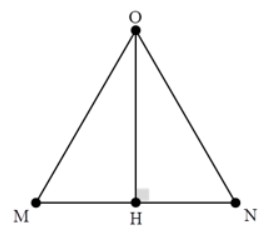
\includegraphics[scale=0.8]{../figs/VN12-PH-13-P-009-1-Q20.jpg}
	\end{center}
	
	Mức cường độ âm máy thu có thể thu được lớn nhất tại điểm H là hình chiếu của O lên MN.
	
	Ta có $\dfrac{\text{OH}}{\text{OM}}=\dfrac{\sqrt{3}}{2}$.
	
	Mức cường độ âm tại H là $L_\text{H}=L_\text{M}+20\log\dfrac{\text{OM}}{\text{OH}}=\SI{16}{dB}$
	

	
	
}
\end{enumerate}
\loigiai{\textbf{Đáp án}
	\begin{center}
		\begin{tabular}{|m{2.8em}|m{2.8em}|m{2.8em}|m{2.8em}|m{2.8em}|m{2.8em}|m{2.8em}|m{2.8em}|m{2.8em}|m{2.8em}|}
			\hline
			1. A & 2. C & 3. C & 4. C & 5. C & 6. A  & 7. B  & 8. D & 9. A & 10. A\\
			\hline
			11. C & 12. D & 13. B & 14. C & 15. D & 16. D  & 17. B  & 18. C & 19. A & 20. C\\
			\hline
		\end{tabular}
\end{center}}